\documentclass[a4paper, 12pt, oneside]{extarticle}
%-shell-escape % якщо використовуєте minted
\input{$HOME/Templates/lpnu_doc_templates/settings/preamble.tex}
% якщо домахуються дуже за Times New Roman, то
% використовуєте xelatex і цей файл:
\input{$HOME/Templates/lpnu_doc_templates/settings/font_styles.tex}
\graphicspath{{images/}}

\newcommand\Variant{12}
\newcommand\Date{12.05.\the\year}
\newcommand\Discipline{Комп'ютерна схемотехніка та архітектура комп'ютерних систем}
\newcommand\Instructor{Чкалов О. В.}

\newcommand\Type{\Lab}
\newcommand\Number{1}
\newcommand\Topic{ОСНОВИ РОБОТИ В ПРОГРАМІ NI MULTISIM }

\usepackage{pgfplotstable}

\pgfplotstableset{
	col sep=tab,
	%trim cells=false,
    header=true,
    string type,
    before row=\hline,
    every last row/.style={after row=\hline},
    column type/.add={|}{},
    every last column/.style={column type/.add={}{|}}
}

\begin{document}
\Margins

\Margins
%\begin{wrapfigure}[3]{l}{.27\textwidth}
%\includegraphics[width=.28\textwidth]{$UNI/.templates/lpnu_logo.png}
%\end{wrapfigure}

%\noindent\textbf{Прізвище:} \Lname \\
%\noindent\textbf{Ім'я:} \Fname \\
%\noindent\textbf{Група:} \Group \\
%\noindent\textbf{Варіант:} \Variant \\
%\noindent\textbf{Дата захисту:} \Date \\
%\\
%\noindent\textbf{Кафедра:} \Department \\
%\noindent\textbf{Дисципліна:} \Discipline \\
%\noindent\textbf{Перевірив:} \Instructor \\

%%\medskip\bigskip

%\begin{center}
%	\textbf{ЗВІТ}		\\
%	до \Type~\No\Number	\\
%	на тему ``\Topic''	\\
%\end{center}

% \begin{table}
%   \begin{tabularx}{\textwidth}{|c|X|X|}
%     \hline
%     % Image & Content & Additional Info \\
%     % \hline
% 	  \multirow{3}{*}{\includegraphics[width=4cm]{$UNI/.templates/lpnu_logo.png}}
% 	  & \textbf{ЗВО:}
% 	  Національний університет ``Львівська Політехніка''.
% 	  & \textbf{Тема:}
% 	  \Topic
% 	  \\
% 	  & \textbf{Навчальний рік:}
% 	  2023/2024
% 	  & \textbf{Інститут}
% 	  комп'ютерних наук та інформаційних технологій
% 	  \\
% 	  & \textbf{Семестр:}
% 	  осінній
% 	  & \textbf{Група:}
% 	  \Group
% 	  \\
% 	  & \textbf{Навчальна дисципліна:}
% 	  \Discipline
% 	  & \textbf{Студент:}
% 	  Мілюхін Олександр
% 	  \\
% 	  & \textbf{Кафедра}
% 	  систем автоматизованого проектування
% 	  &
% 	  \\
% 	  & \textbf{Викладач:}
% 	  Чумакевич В. В.
% 	  &
% 	  \\
%     \hline
%   \end{tabularx}
% \end{table}

\setlength{\textfloatsep}{-16pt}
% \setlength{\intextsep}{0pt}

\begin{table}
	\begin{tabular}{|l|l|p{6cm}|}
    \hline
    % Image & Content & Additional Info \\
    % \hline
	  \makecell[l]{
	  \includegraphics[width=3.37cm]{$UNI/.templates/lpnu_logo.png}
  }
	  & \makecell[l]{
	  \textbf{ЗВО:}
	  Національний університет \\ ``Львівська Політехніка''.
	  \\
	  \textbf{Навчальний рік:}
	  2023/2024
	  \\
	  \textbf{Семестр:}
	  осінній
	  \\
	  \textbf{Навчальна дисципліна:} \\
	  \Discipline
	  \\
	  \textbf{Кафедра}
	  систем автоматизованого \\ проектування
	  \\
	  \textbf{Викладач:}
	  Чумакевич В. В.
}
	  & \makecell [l] {
	  \textbf{Тема:}
	  \Topic
	  \\
          \textbf{Інститут}
	  комп'ютерних наук та \\ інформаційних технологій
	  \\
	  \textbf{Група:}
	  \Group
	  \\
	  \textbf{Студент:}
	  Мілюхін Олександр
  }
  \\
    \hline
  \end{tabular}
\end{table}
\section{Мета роботи}

% \begin{table}
%   \begin{tabularx}{\textwidth}{|p{6cm}|c|c|}
% 	  \hline
%     \multirow{3}{*}{\includegraphics[width=6cm]{$UNI/.templates/lpnu_logo.png}}
% 	  & ЗВО: Національний університет ``Львівська Політехніка''
% 	  & Additional Info 1 \\
%     & Content 2 & Additional Info 2 \\
%     & Content 3 & Additional Info 3 \\
% 	  \hline
%   \end{tabularx}
% \end{table}

% \begin{table}
%   \begin{tabular}{|c|c|c|}
%     \hline
%     \multirow{3}{*}{\includegraphics[width=3cm]{$UNI/.templates/lpnu_logo.png}} & \makecell{Content 1 \\ Content 2 \\ Content 3} & \makecell{Additional Info 1 \\ Additional Info 2 \\ Additional Info 3} \\
%     \hline
%   \end{tabular}
% \end{table}


ознайомлення з інтерфейсом та основними можливостями
програми NI Multisim.

\section*{Індивідуальне завдання}

\subsection*{Завдання 1}

Визначити опір ділянки кола. Принципові схеми для
розрахунку опору ділянки кола приведені в табл. 1.1, варіанти завдань і
номінали резисторів -  в табл. 1.2.

\begin{figure}[h]
	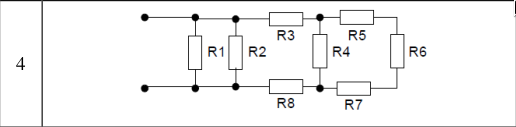
\includegraphics[width=.5\textwidth]{task1}
\end{figure}

\begin{table}[h]
\pgfplotstabletypeset{1.1}%
\end{table}

\subsection*{Завдання 2}

 Визначити струми, які протікають через опори R1-R6 та спад
напруги на них. Принципові схеми для проектування приведені в табл. 1.3,
варіанти завдань і номінальні значення резисторів та ЕРС джерел в табл. 1.4.

\begin{figure}[h]
	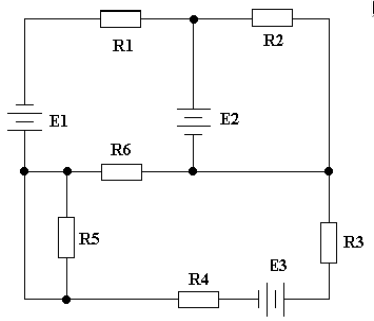
\includegraphics[width=.3\textwidth]{task2}
\end{figure}

\begin{table}[h]
\pgfplotstabletypeset{3r2}%
\end{table}

\subsection*{Завдання 3}

А – амплітуда,  – частота сигналу; КЗ – коефіцієнт
заповнення.

\begin{figure}[h]
	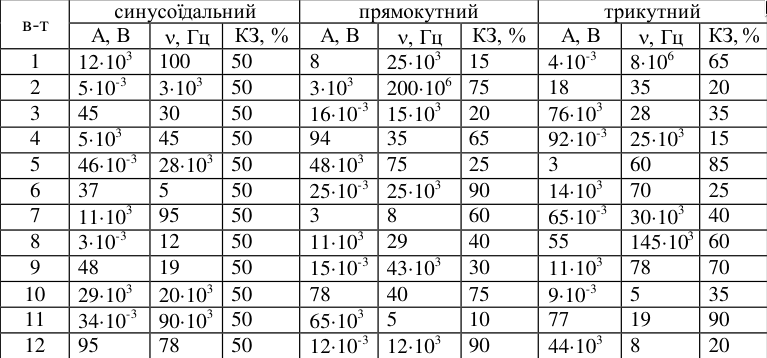
\includegraphics[width=.8\textwidth]{images/task3.png}
\end{figure}

\section*{Етапи розв'язку}

\subsection*{Завдання 1}
% \begin{figure}[h]
% 	\centering
	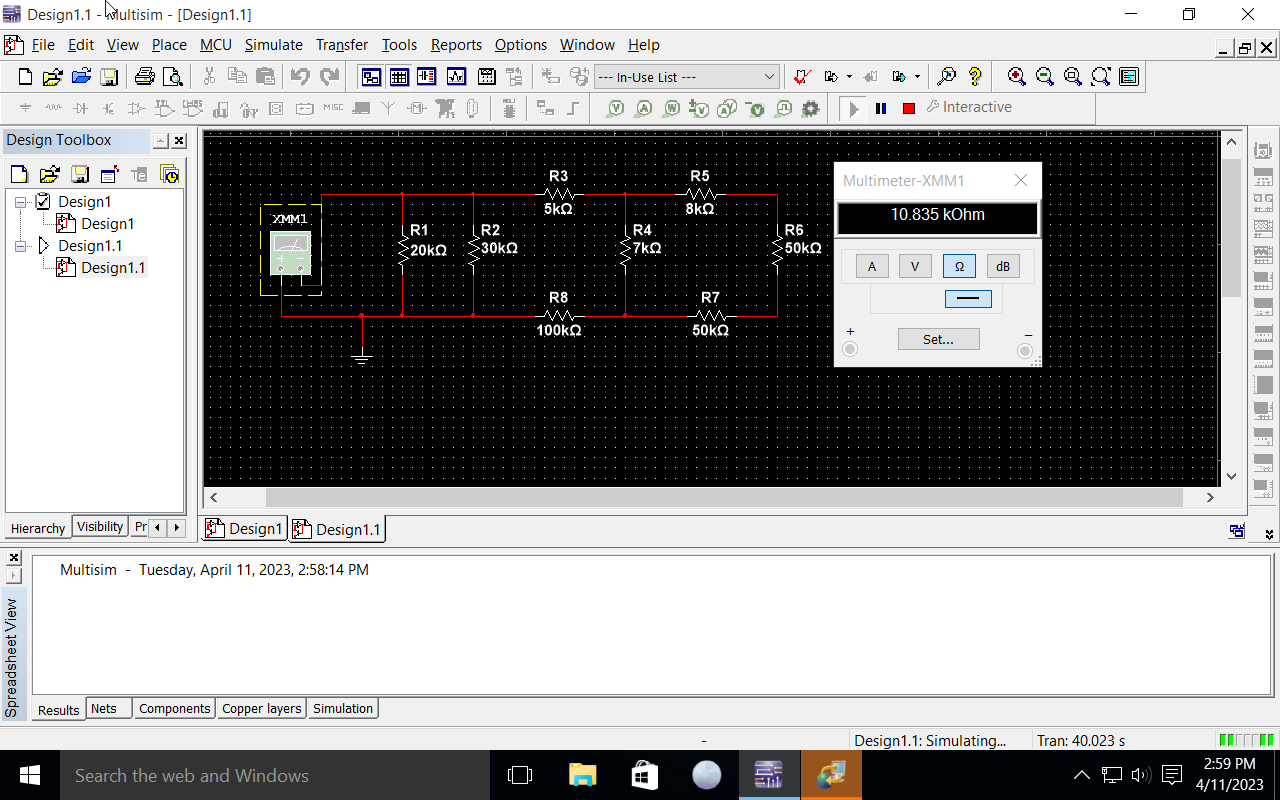
\includegraphics[width=\textwidth]{1.1.res}
	% \caption{знімок екрану зі схемою й даними мультиметра}
% \end{figure}

\begin{align}
8+50+50 = 108 \\
1/108 + 1/7 = .15211640211640211639 \\
1/0.152116 = 6.57393042152041862788 \\
1/30+1/20+1/6.57393 = .23544934308701187873 \\
1/.2 = 5\\
1/0.152116+105 = 111.57393042152041862788 \\
1/30+1/20+1/111 = .09234234234234234233 \\
1/.09 = 11.11111111111111111111
\end{align}

\subsection*{Завдання 2}
\begin{figure}[h]
	\centering
	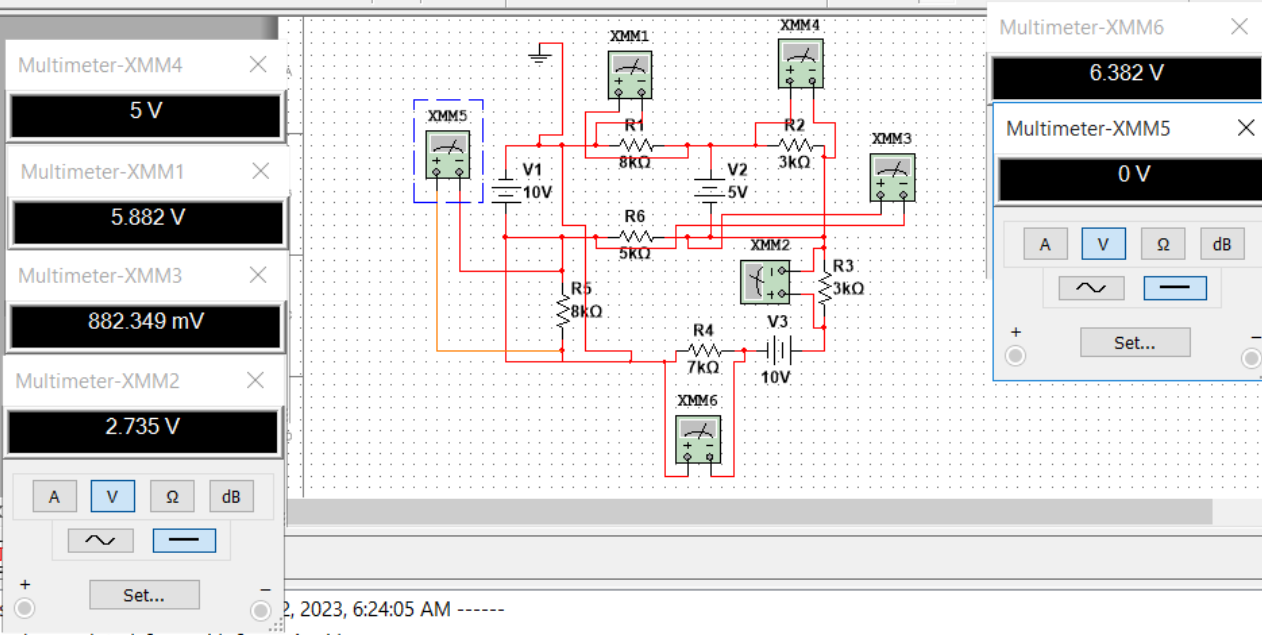
\includegraphics[width=.9\textwidth]{task2res}
	\caption{Виміри спадів напруги}
\end{figure}
\begin{figure}[h]
	\centering
	% 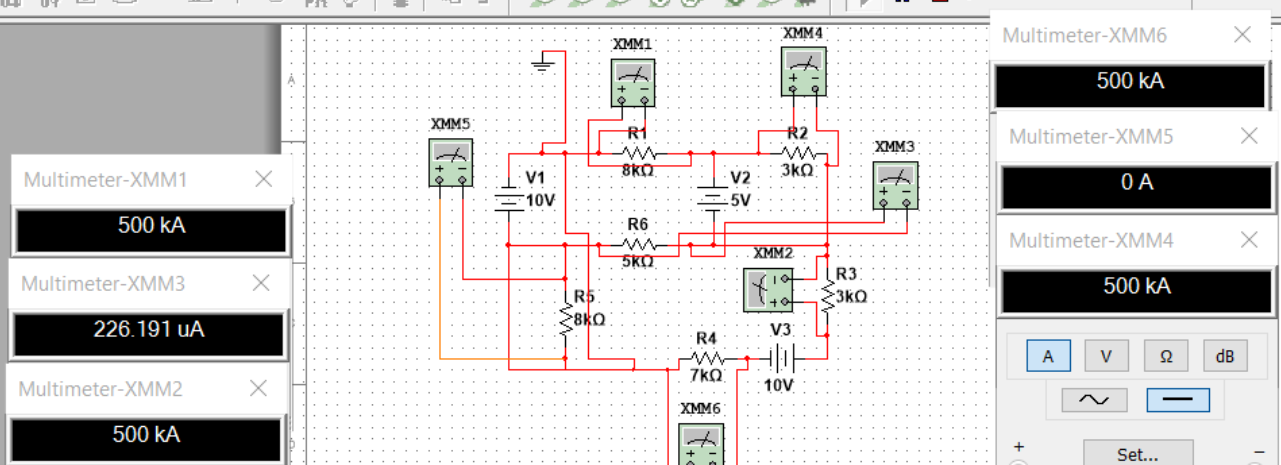
\includegraphics[width=.9\textwidth]{task2imp}
	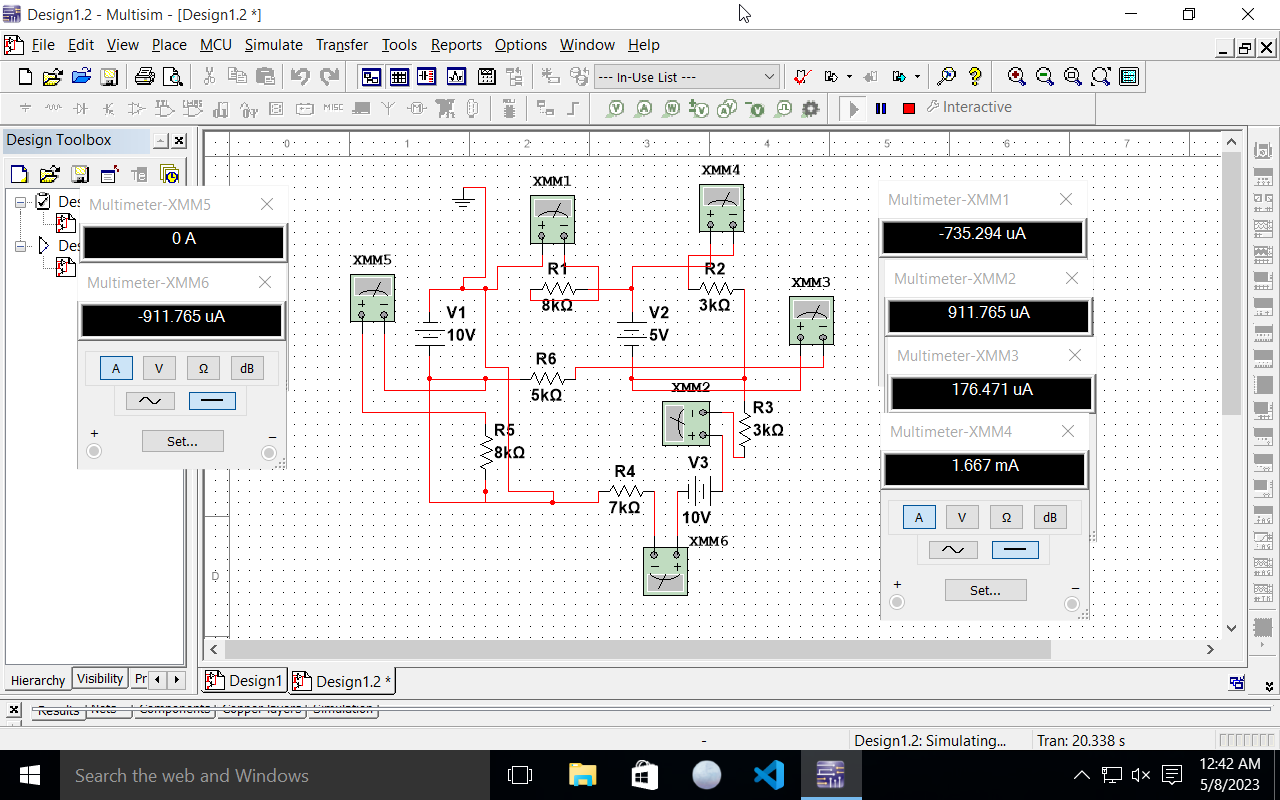
\includegraphics[width=.9\textwidth]{strum}
	\caption{Виміри струму}
\end{figure}

\begin{table}[h]
%\pgfplotstabletypeset{t2results}%
\end{table}

\subsection*{Завдання 3}
\subsubsection*{Синусоїдальний}
	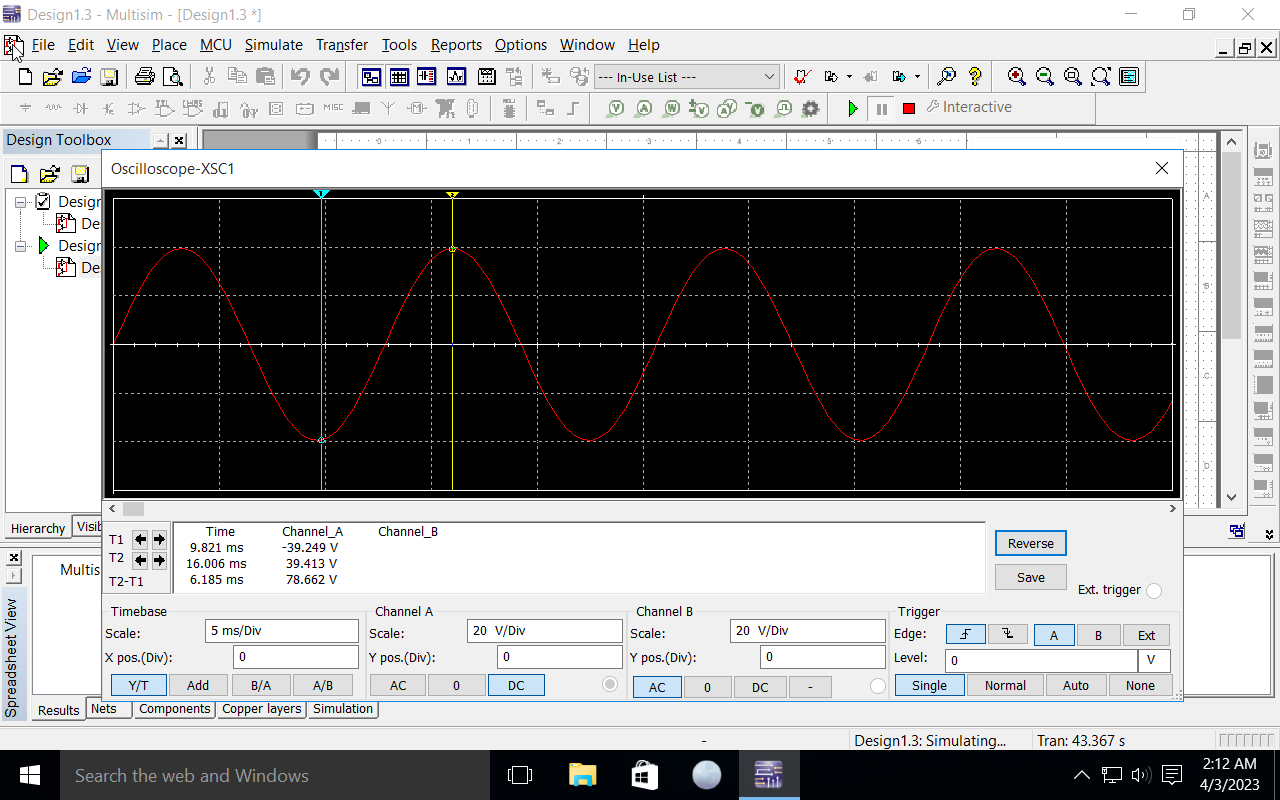
\includegraphics[width=.9\textwidth]{sin}
\subsubsection*{Прямокутний}
\begin{figure}[ht]
	\centering
	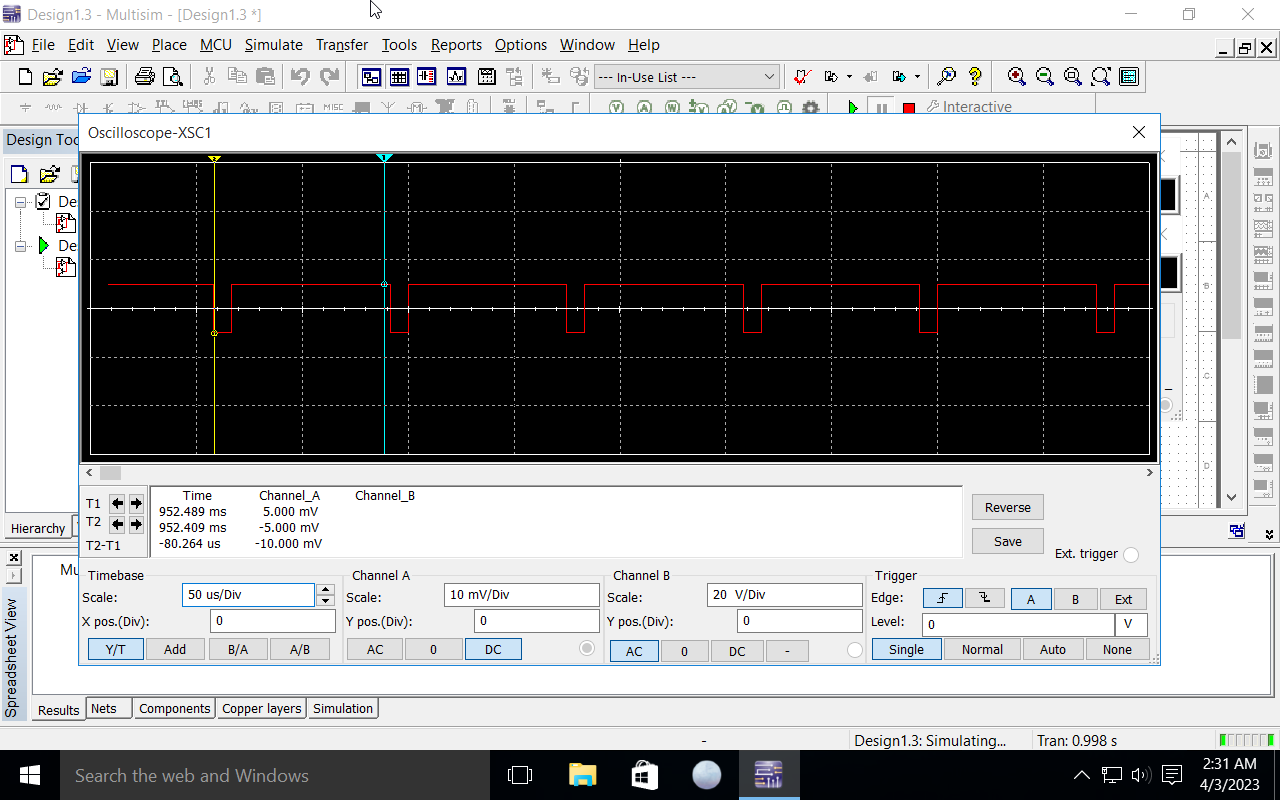
\includegraphics[width=.9\textwidth]{rec2}
	\caption{амплітуда}
\end{figure}
\begin{figure}[t]
	\centering
	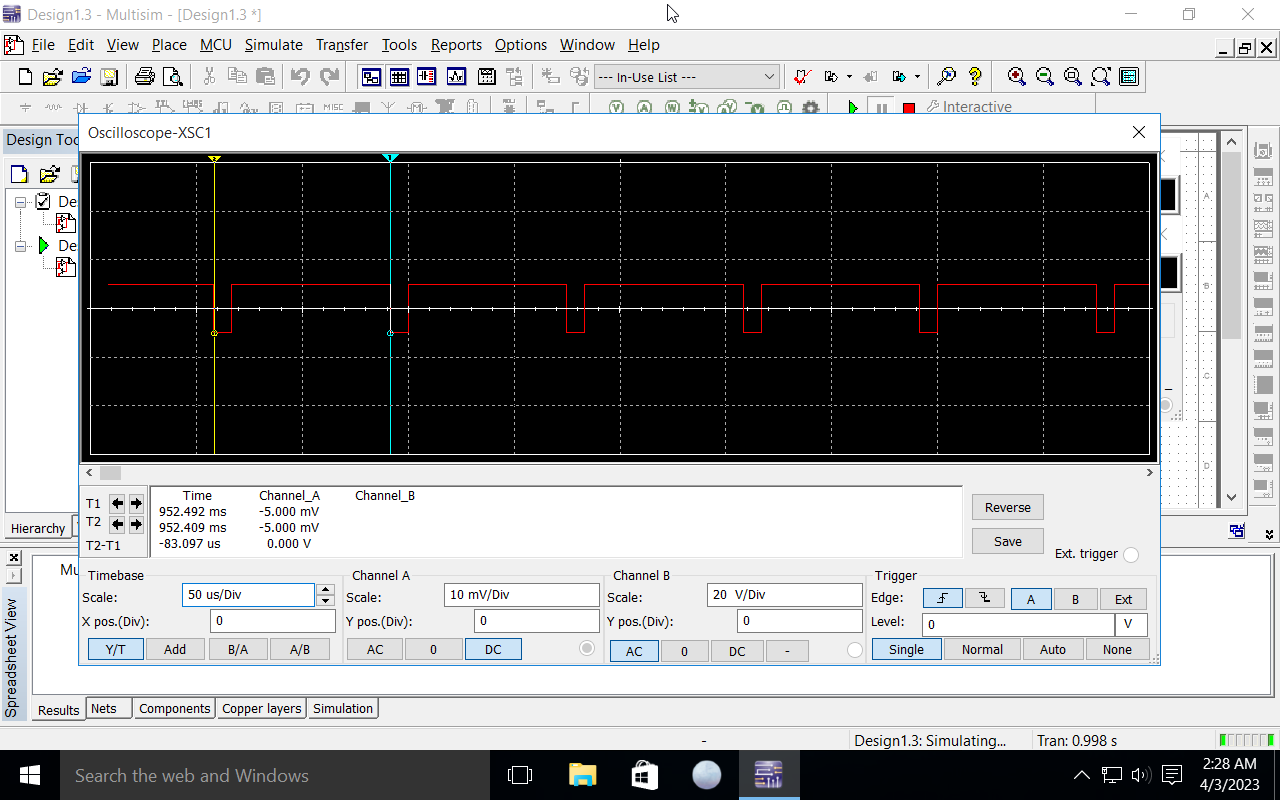
\includegraphics[width=.9\textwidth]{rec1}
	\caption{період}
\end{figure}
\clearpage
\subsubsection*{трикутний}
\begin{figure}[h]
	\centering
	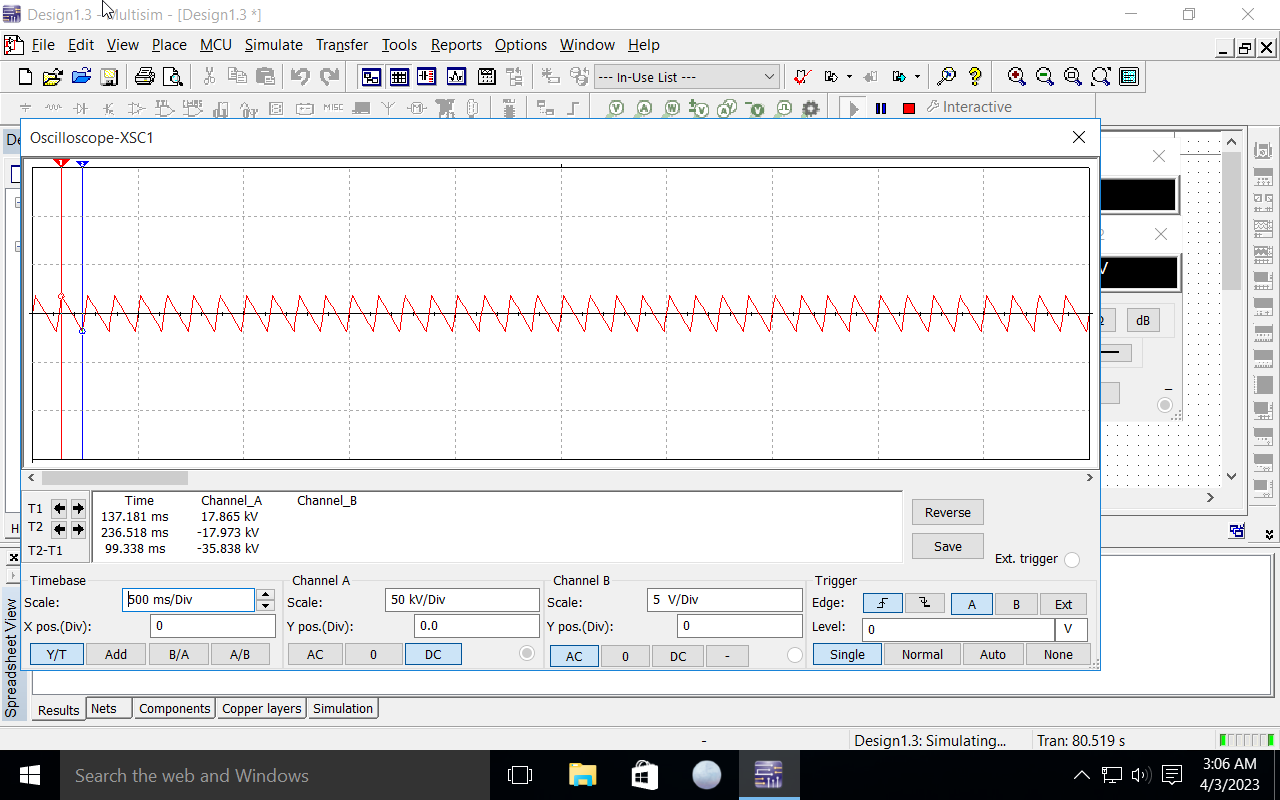
\includegraphics[width=.9\textwidth]{tri1}
	\caption{амплітуда}
\end{figure}
\begin{figure}[h]
	\centering
	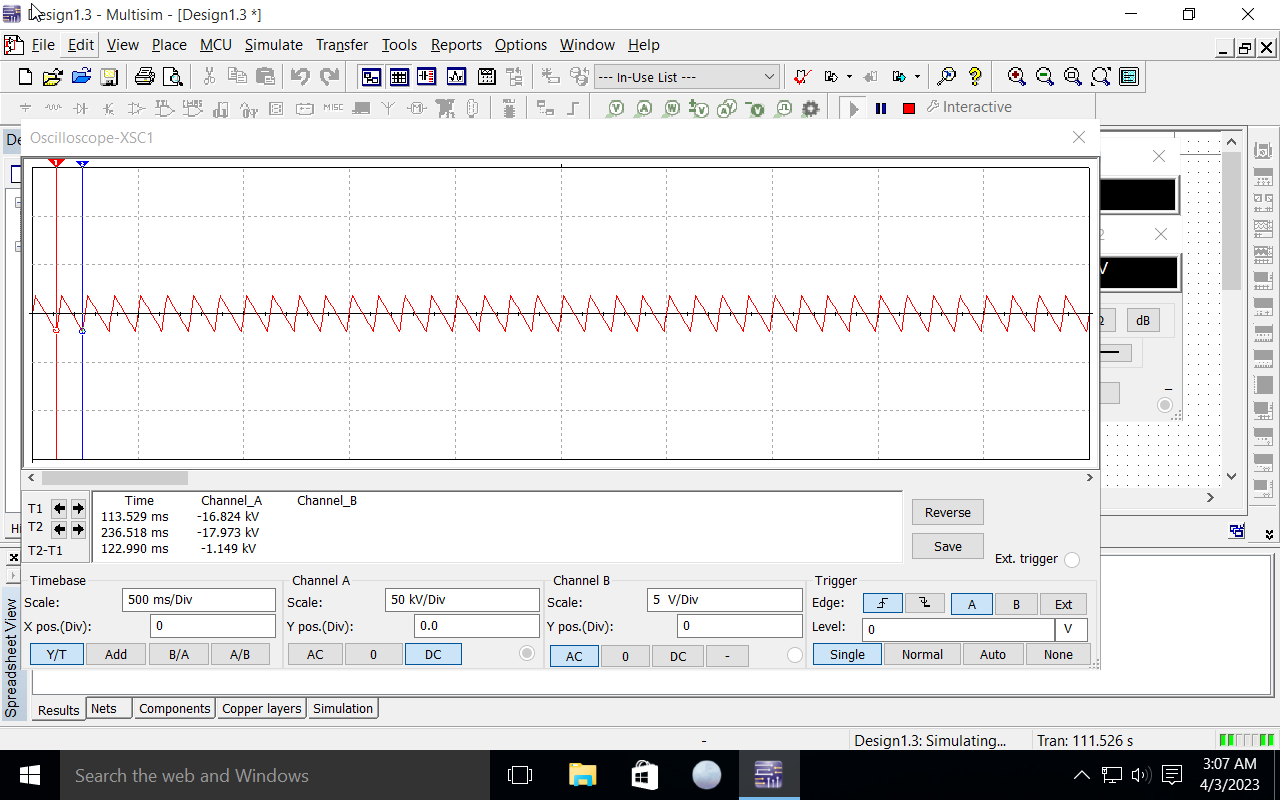
\includegraphics[width=.9\textwidth]{tri2}
	\caption{період}
\end{figure}

\begin{table}[h]
\pgfplotstabletypeset{3res}%
\end{table}

\clearpage

\section*{Висновок}

Виконуючи цю лабораторну роботу, я навчився основам
побудови схем у програмі NI Multisim.

\section*{Відповіді на контрольні запитання}
\begin{itemize}
	\question Які величини можуть бути виміряні мультиметром?
	\answer Сила струму, напруга, опір, потужність сигналу.

	\question Як виконати поворот елемента у програмі NI Multisim?
		\answer Ctrl+[Shift]+R

	\question Скільки з'єднань можна підвести до одного з'єднувального вузла (конектора) у програмі NI Multisim?
	\answer залежить від налаштувань програми та типу вузла, у стандартному --- до 16 провідників.

	\question Яким чином змінюється номінальне значення опору резистора, які ще параметри резистора можна задати.
	\answer використовуючи панель властивостей (Properties Panel) для вибраного резистора. Крім того, в цьому вікні можна задати інші параметри резистора, такі як точність, потужність, температурний коефіцієнт опору та інші.

	\question При вимірюванні опору мультиметром в колі створюється деякий струм. Чи впливає величина цього струму на результат вимірів?
	\answer Так, але зазвичай дуже несуттєво

	\question Якими способами можна з'єднати два джерела струму, пояснити, як визначається результуюча ЕРС для кожного способу з'єднання.
	\answer
		\begin{itemize}
			\item	Послідовне з'єднання: джерела струму з'єднуються послідовно одне з одним, так що струми проходять через коло по черзі. В такому випадку результуюча ЕРС (EMF) дорівнює сумі ЕРС двох джерел струму. %Згідно з законом Кірхгофа про послідовне з'єднання джерел, результуючий струм дорівнює струму в кожному джерелі струму.
			\item
Паралельне з'єднання: джерела струму з'єднуються паралельно одне з одним, так що струми розділяються на декілька шляхів. У такому випадку результуюча ЕРС дорівнює ЕРС одного з джерел струму. %Згідно з законом Кірхгофа про паралельне з'єднання джерел, результуючий струм дорівнює сумі струмів, що протікають через кожне з джерел струму.
		\end{itemize}

	\question Чи можна виміряти внутрішній опір  джерела струму, як це зробити?
	\answer Так. Для цього можна скористатися функцією "AC Analysis" (аналіз постійної складової) та додати до схеми вимірювальний опір.

	\question Як виміряти потенціал довільної точки в розгалуженому електричному колі, яке містить декілька джерел струму.
	\answer У NI Multisim для вимірювання потенціалу довільної точки в розгалуженому електричному колі можна використовувати вбудовану функцію вимірювання напруги (Voltage Probe).
\end{itemize}
\end{document}
